%
% File acl2018.tex
%
%% Based on the style files for ACL-2017, with some changes, which were, in turn,
%% Based on the style files for ACL-2015, with some improvements
%%  taken from the NAACL-2016 style
%% Based on the style files for ACL-2014, which were, in turn,
%% based on ACL-2013, ACL-2012, ACL-2011, ACL-2010, ACL-IJCNLP-2009,
%% EACL-2009, IJCNLP-2008...
%% Based on the style files for EACL 2006 by
%%e.agirre@ehu.es or Sergi.Balari@uab.es
%% and that of ACL 08 by Joakim Nivre and Noah Smith

\documentclass[11pt,a4paper]{article}
\usepackage[hyperref]{acl2018}
\usepackage{times}
\usepackage{latexsym}
\usepackage{tikz}
\usepackage{pgfplots}
\usepackage{multirow}
\usepackage{url}
\usepackage{graphicx}
\usepackage{amsmath}
\usepackage{pgfplots}
\usepackage{array,ragged2e}
\usepackage{textcomp}
\usepackage{pgfplotstable}
\usepackage{enumitem}
\setlist{itemsep=0pt}

%\aclfinalcopy % Uncomment this line for the final submission
%\def\aclpaperid{***} %  Enter the acl Paper ID here

%\setlength\titlebox{5cm}
% You can expand the titlebox if you need extra space
% to show all the authors. Please do not make the titlebox
% smaller than 5cm (the original size); we will check this
% in the camera-ready version and ask you to change it back.

\newcommand\BibTeX{B{\sc ib}\TeX}

\title{Fat Encoder, Thin Decoder \protect\\ OpenNMT System Description for WNMT 2018}

\author{First Author \\
  Affiliation / Address line 1 \\
  Affiliation / Address line 2 \\
  Affiliation / Address line 3 \\
  {\tt email@domain} \\\And
  Second Author \\
  Affiliation / Address line 1 \\
  Affiliation / Address line 2 \\
  Affiliation / Address line 3 \\
  {\tt email@domain} \\}

\date{}

\begin{document}
\maketitle
\begin{abstract}
In this paper, we present OpenNMT sequence to sequence neural machine translation (NMT) system for the WNMT 2018 evaluation optimized for CPU inference. This work led to development of new features that have been integrated to OpenNMT and already available to the community.

\end{abstract}

\section{Introduction}
In this paper, we describe the systems we built and selected for WNMT 2018\footnote{\url{https://sites.google.com/site/wnmt18/shared-task}}. Our specific interest was to explore the different techniques for training and optimizing CPU models with high throughput while keeping high accuracy. Even though we did not put real focus on memory and docker size footprint, we applied basic optimization techniques to reduce the final size of our models (delivered as fully functional dockers).

For this purpose, we explored the following techniques:
\begin{itemize}
\item Model distillation as introduced by \newcite{distillation} to transfer knowledge from a strong baseline neural network (the teacher) to a smaller network (the student); we were in particular interested to explore the possibility of distilling knowledge from a transformer model \cite{vaswani2017attention} to a light-weight RNN model,
\item Changing the structure of the network by increasing the size of more efficient modules, reducing the size of the more costly, and replacing default gated units,
\item Using C++ based decoder \textit{CTranslate}\footnote{\url{https://github.com/OpenNMT/CTranslate}},
\item Reducing dynamically the runtime target vocabulary extending \cite{shi2017speeding} ideas,
\item Quantizing parameters of the models as presented in \newcite{DBLP:journals/corr/Devlin17} or {\tt gemmlowp}\footnote{\url{https://github.com/google/gemmlowp}}
\end{itemize}

The complete training workflow is therefore based on the following steps:
\begin{itemize}
\item Preparation of data and sub-tokenization model - described in section \ref{data}.
\item Training of strong a Teacher transformer model, and translation of the full dataset with this model - described in section \ref{transformer}.
\item Training of student model on translated data - described in section \ref{distill} and \ref{seq2seq}.
\item Quantizing the generated model - described in section \ref{quantize}.
\end{itemize}

\begin{figure}
\scalebox{0.9}{
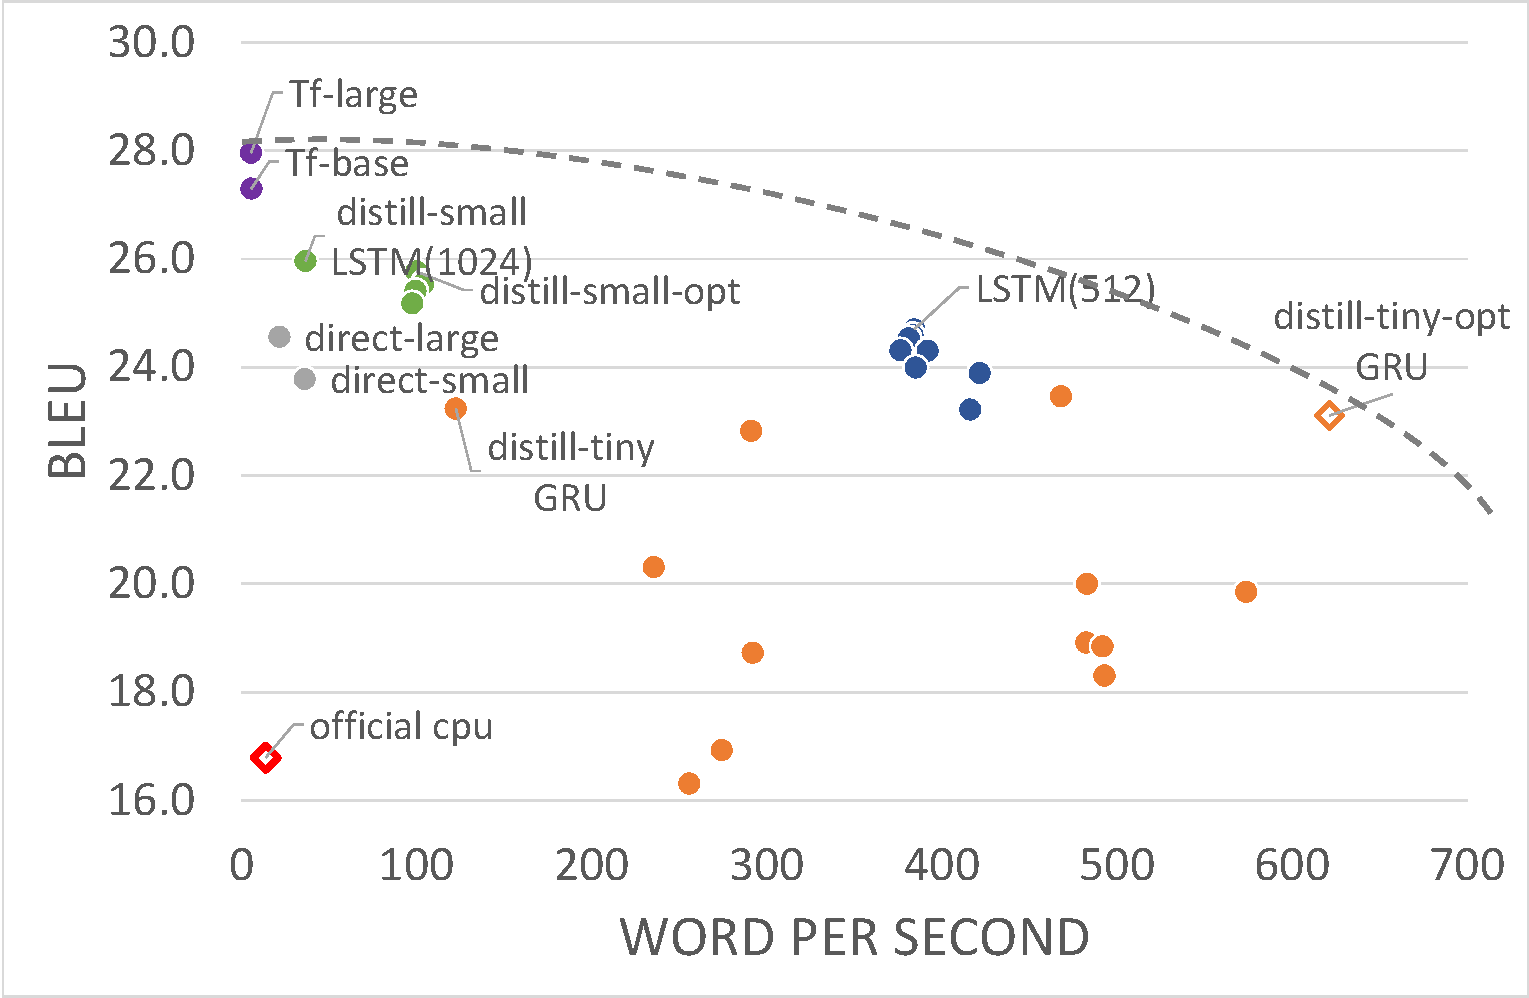
\includegraphics[width=\linewidth]{pareto.pdf}
}
\caption{Pareto on accuracy and throughput.}
\label{fig:pareto}
\end{figure}

By combining all these techniques, we generated a large number of models and picked two of them presenting interesting trade-off between speed and quality and on the frontier of the Pareto curve (see Figure \ref{fig:pareto}). Our first system {\tt LSTM-opt-2} is a simple 2-layer LSTM network is only -2.19 points behind reference transformer model, with a speed-up of \textcolor{red}{x18}. Our second system achieves 23.11 on WNMT 2018 English-German newstest2014 (-4.85 behind the reference model) but  with an additional decoding speed-up of \textcolor{red}{x6} at about 1000 words/sec on the evaluation hardware.

Also, we show that distillation of transformer model outperforms training result of a strong RNN model - extending findings of \cite{DBLP:journals/corr/CregoS16} who reported that student systems could outperform their teacher for reference RNN-based model.

Finally, we also report several other negative experiments that produced systems inside of the pareto convex border. For instance, we compared using 8-bit quantization to 16-bit quantization.

Beyond the presented systems, this paper brings the following contributions: a/ we prove that distillation from a transformer neural network to a simple RNN neural network is efficient, b/ we compare quantitatively different quantizations, c/ we improve algorithm to select dynamically target vocabulary for a given batch.

\begin{table*}[]
\centering
\begin{tabular}{lccccrr}
\hline
                    & \multicolumn{1}{l}{\(\displaystyle N \)} & \multicolumn{1}{l}{\(\displaystyle d_{model} \)} & \multicolumn{1}{l}{\(\displaystyle d_{ff} \)} & \multicolumn{1}{l}{\(\displaystyle h \)} & \multicolumn{1}{l}{newstest2014} & \multicolumn{1}{l}{newstest2015} \\ \hline
Transformer (base)  & 6                     & 512                        & 2048                  & 8                        & 27.30                            & 29.36                            \\ \hline
Transformer (large) & 6                     & 512                        & 4096                  & 8                        & 27.96                            & 29.95                            \\ \hline
\end{tabular}
\caption{Evaluation on transformer based teacher system}
\label{table:transformer}
\end{table*}

\section{Training}

\subsection{Data}
\label{data}

We use constrained data set provided by WNMT 2018, which is a preprocessed and tokenized version of WMT 2014 on English-German translation\footnote{\url{https://nlp.stanford.edu/projects/nmt/}}. The training data contains about 4.5M sentence pairs. We use newstest2013 as the validation set and newstest2014 and newstest2015 as the testing sets. Before training, we trained a 32K joint byte-pair encoding (BPE) to preprocess the data \cite{sennrich2015neural}. Hence, the generated subword vocabulary is less than 40K word pieces. And we limit the sentence length to 100 based on BPE preprocessing in both source and target side (excluding only $0.31\%$ of the training corpus). After decoding, we remove the BPE joiners and evaluate the tokenized output with multi-bleu.perl\footnote{\url{https://github.com/moses-smt/mosesdecoder/blob/master/scripts/generic/multi-bleu.perl}}.

\subsection{Transformer}
\label{transformer}
% teacher system
We train a transformer based system \cite{vaswani2017attention} as our teacher system.
Compared with RNN/CNN models, transformer based model does not rely on recurrent or convolution network.
It directly models the representations of each sentence with self-attention mechanism.
Hence much longer information in the sentences can be learned especially important for language pairs like English-German and it currently achieves state-of-art results for machine translation \cite{DBLP:journals/corr/abs-1803-02155}

Another advantage for transformer based system is that the training process can be parallelized easily.
However, transformer networks still require a large number of parameters and also large memory to achieve the best performance.
As a result, the parallelizable training, the flexibility in modeling both long-range/local
dependencies, and the state-of-the-art performance make this architecture suitable to act as the teacher system.

We used \textit{OpenNMT-tf}\footnote{\url{https://github.com/OpenNMT/OpenNMT-tf}} to train two transformer based systems: base and large described in table \ref{table:transformer} with their evaluation. For both, the learning rate is set to 2.0 and warmup steps 8000, we average the last 8 checkpoints to get the final model. Our baseline system outperforms in particular the provided baseline sockeye model with +0.37 BLEU on newstest 2014.

\subsection{Distillation}
\label{distill}

We follow the method described in \newcite{distillation}. Firstly, we build the full transformer based MT system \cite{vaswani2017attention} as the teacher system. Secondly, we use the teacher system to translate all the source sentences to generate a simplified target sentences set.
Then, we use this simplified corpus (original source and newly generated target) to train a student system, in our case a sequence-to-sequence models similar to \newcite{bahdanau2014neural}.
The student system can be assigned with smaller network size and this process is called distillation.

According to \newcite{DBLP:journals/corr/CregoS16}, distillation process not only improves throughput of the models and reduce their size, but can also improve the translation quality if the width of the network is not reduced too much. Also, these distilled systems have the interesting feature that they performed almost identically for beam 2 or beam 5 beam search. The interpretation for these facts being that the teacher produced simplified translations. That is, translations that are usually closer, in terms of syntactic structure and even word choices, to the input sentences than reference translations. Thus the student model better manage to learn and generalize this simplified knowledge. One major question here was to find out whether distillation from an transformer model could benefit a student RNN model. We proved it was the case, since the best distilled system outperforms a larger model trained with the original data.

\subsection{Sequence to Sequence}
\label{seq2seq}

Our baseline NMT system follows the architecture presented in ~\newcite{luong-pham-manning:2015:EMNLP}. It is implemented as an encoder-decoder network with multiple layers of a RNN with Long Short-Term Memory hidden units ~\cite{DBLP:journals/corr/ZarembaSV14} and attentional architecture from ~\newcite{luong-pham-manning:2015:EMNLP} available on \textit{OpenNMT}\footnote{\url{https://github.com/OpenNMT/OpenNMT}}. Full details of the system are given in \newcite{KleinKDSR17}.
%Additional details are given in \cite{DBLP:journals/corr/CregoKKRYSABCDE16}.

\begin{figure}
\scalebox{0.9}{
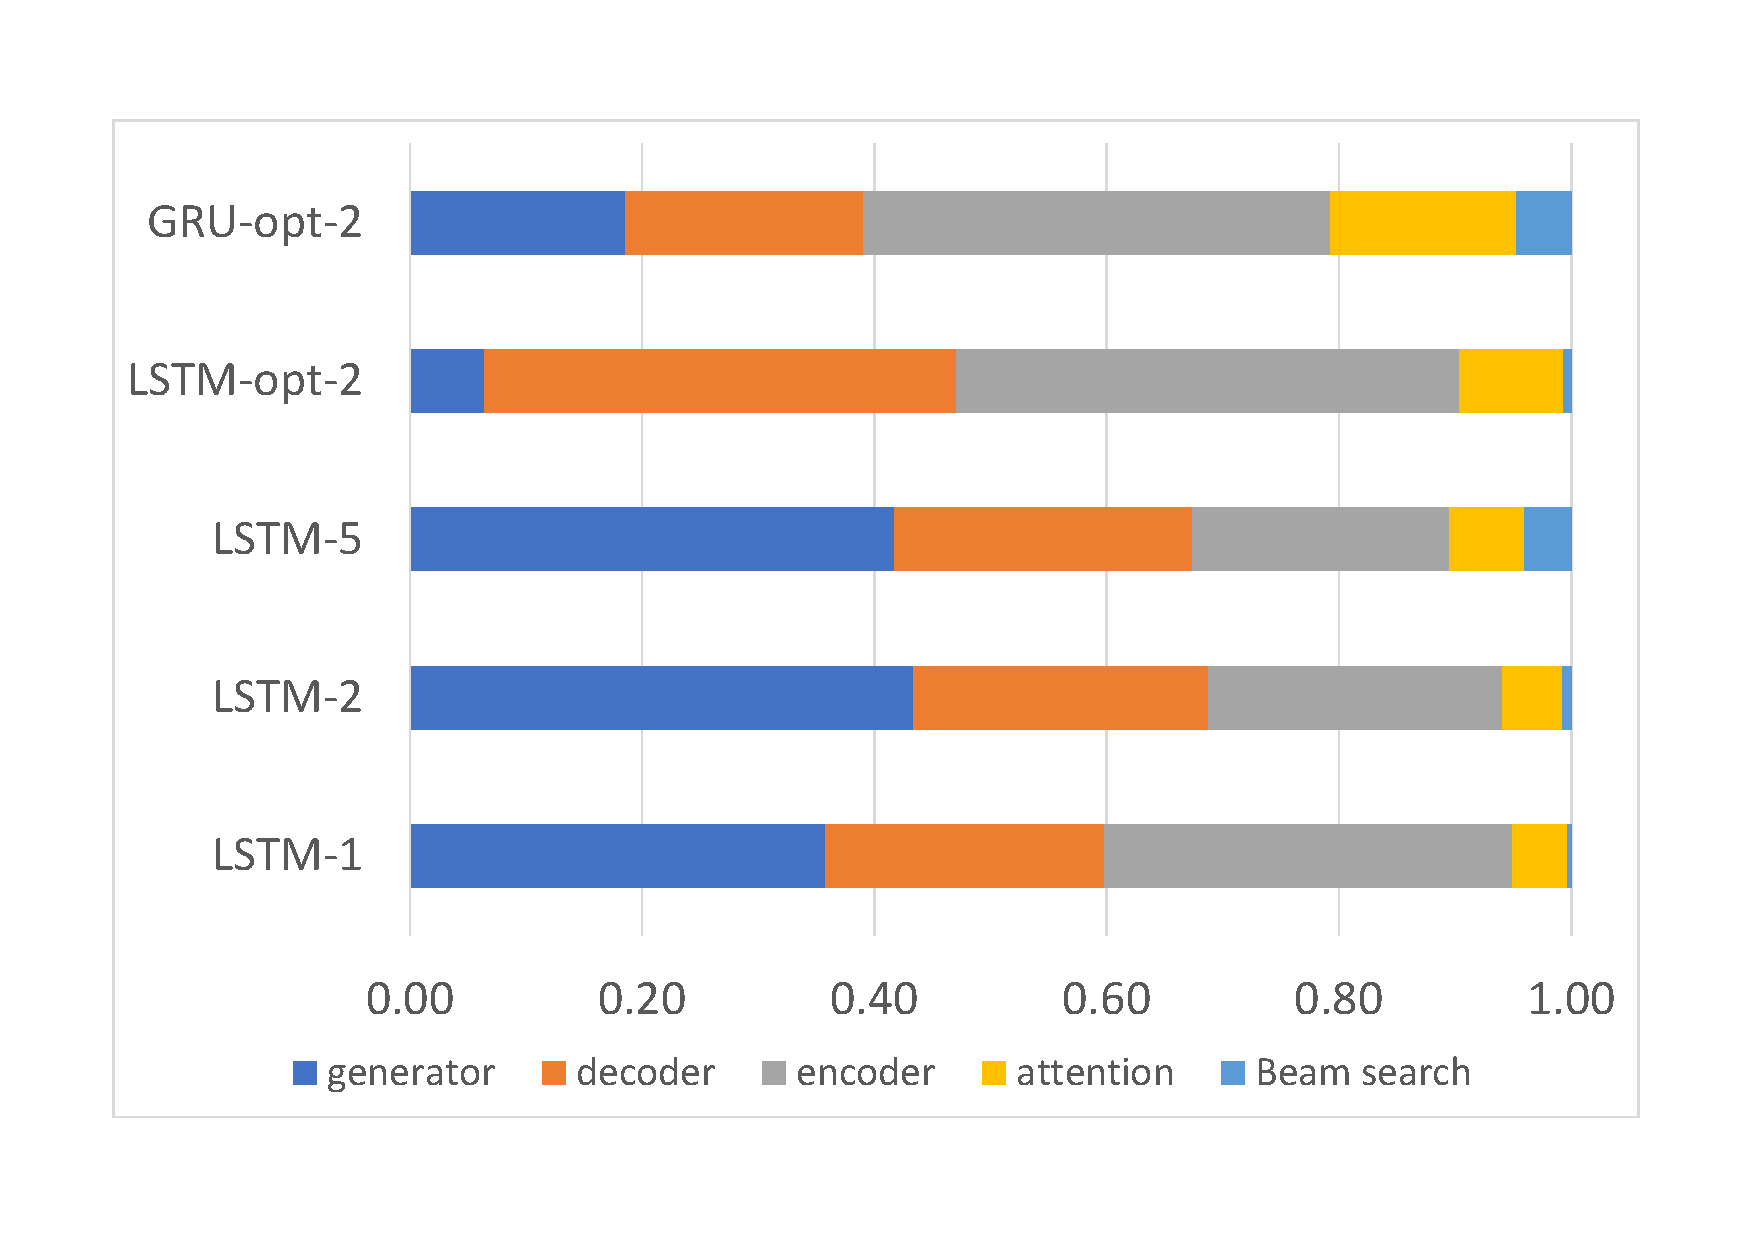
\includegraphics[width=\linewidth]{decoder.pdf}
}
\scalebox{0.9}{
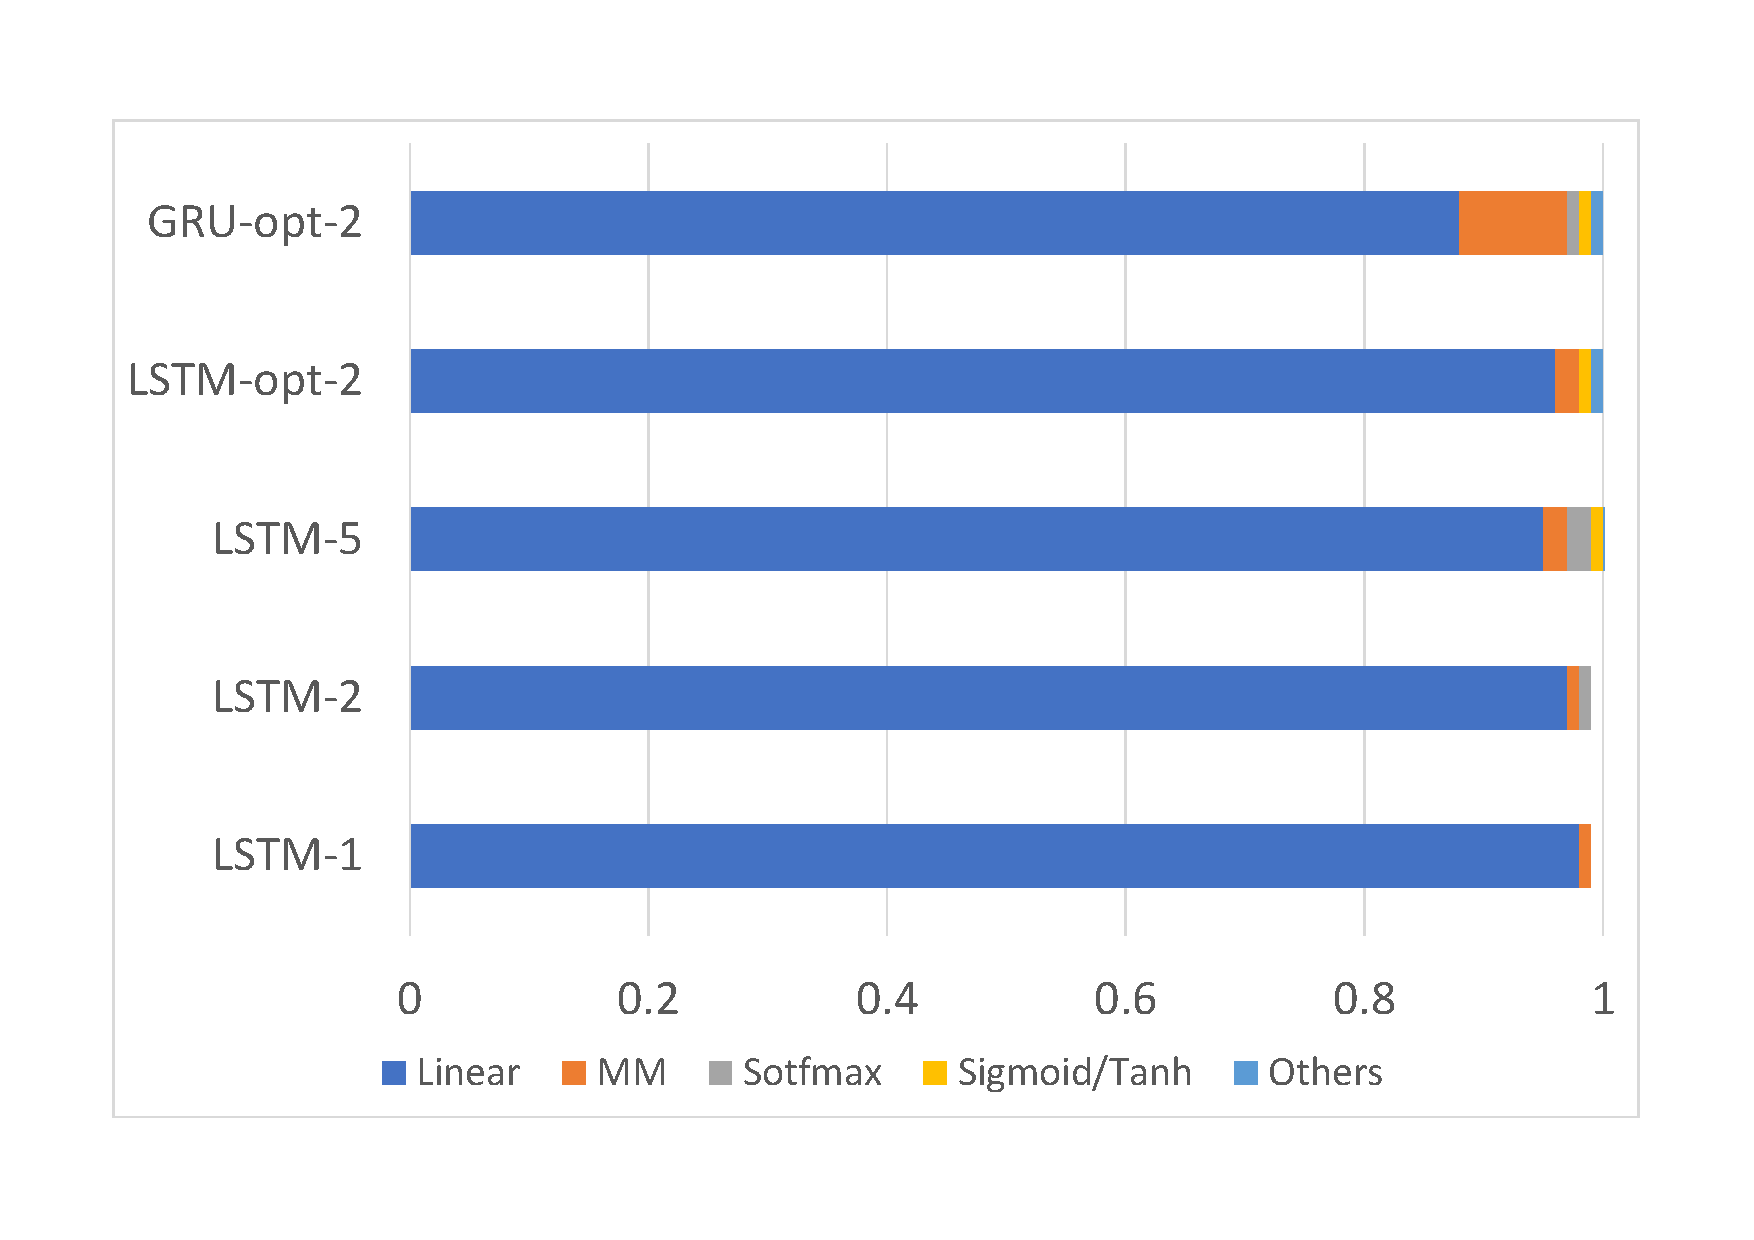
\includegraphics[width=\linewidth]{decoder_linear.pdf}
}
\caption{Profiling of the throughput during inference of newstest2014. Each line is a different system. The {\tt LSTM-1,2,5} are baseline systems with respective beam size of 1, 2, 5. {\tt GRU-opt-2} and {\tt LSTM-opt-2} are the presented systems. The total decoding time for each of these systems (in seconds) are from top to bottom: 60, 464, 754, 662 and 629. The top table show the distribution of time per component of the network, while the bottom table show the distribution of time for network operators.}
\label{fig:decoding_cost}
\end{figure}

Profiling of the throughput of such system is presented in Figure \ref{fig:decoding_cost}. From this analysis we gather the following facts:

\begin{itemize}
\item The most costly part of the inference is the generator, that is the final Linear layer feeding Softmax with weights corresponding to each single vocab of the target language. This is by far the largest matrix multiplication of the system: $(B,W) * (W,V)$ (with $B$ being the batch*beam size, $W$ the width of the network, and $V$ the size of the vocabulary).
\item Although the cost of the encoder for beam size 1 is higher than the decoder, the decoder cost - including generator and attention model - grows linearly with the beam size.
\item Transversally to the different component of the network, the most costly module is the Linear module cumulating more 95\% of the complete processing time
\end{itemize}

For these observations, it is obvious that we needed to optimize the efficiency of Linear operation (basic matrix multiplication), reduce their number and have a special focus on the generation layer. It was also interesting to note that focus on any other operator was useless.

On the model architecture, we tried different model combination based on a "fat encoder, thin decoder" spirit: ie. increasing if necessary the number of operations in the encoder part if we can in parallel reduce the number of operations in the decoder.

Also, we tried to substitute LSTM \newcite{Hochreiter:1997:LSM:1246443.1246450} cell with GRU cells \newcite{DBLP:journals/corr/ChoMGBSB14}. Indeed LSTM cells have 4 gates while GRU cells only 3, so potentially leading to a 25\% improvement in speed. We are not aware of any comprehensive study comparing relative efficiency of GRU vs LSTM. Our findings show that almost similar performance can be reached (see figure XX). However, GRU requires more care in optimization method while a naive SGD optimization is generally sufficient for LSTM-RNN trainings.

\section{Decoding optimization}

%introduction is analysis of profiling
%=> fat encoder, thin decoder

% model is Microsoft paper

% no FC -> no convergence?
% full quantized graph
% sigmoid quantizatgio

\subsection{C++ Decoder: CTranslate}

CTranslate is an open source inference engine for OpenNMT models (designed for LuaTorch version) that uses raw C++ with minimal dependencies. The project can load trained models, read the computation graph, and run inference using the popular Eigen library.

CTranslate's goal is to offer a lightweight and embeddable solution for executing models and to support advanced CPU optimization such as quantization and parallel translation. Without these optimization, it still benefits from Eigen efficiency and is about 20\% faster than an Torch application using Intel MKL. Additionally, the use of C++ over a garbage-collected language ensures a predictable and reduced memory usage.


\subsection{Reduction of vocabulary size}
% find reference paper
% our contribution to extend n-gram level
To reduce the size of the vocabulary for each batch, we started up from word alignment method presented in \cite{shi2017speeding}. This approach is essentially a 1-gram approach. However to increase the coverage of the selected meanings without increasing the size of the mapping model, we first extracted words in the target languages that are spontaneously generated (generally without alignment with the source) - e.g. determiners when translating from English to French. We kept the 100 most frequent such words and call them 0-gram meanings. Then we go trough 1-gram, 2-gram, ..., n-grams. For each source phrase $f_1 ... f_n$, we consider the target phrase as a bag of words, and we check the meanings of the covered $0$, ... $n-1$-grams and discard these meanings from the bag of words. If words remain after examining all of the sub-sequence, we consider these words as new meaning for the current phrase. This approach extends vocabulary mapping to multi-word expressions|footnote{For instance {\tt speed test} translated by {\tt test de vitesse} in French is covered by 0-grams, and 1-gram. However, {\tt once more} translated by {à nouveau} will need 2 additional meanings not covered in 0-gram or 1-gram meanings}. We have multiple criterion to extract a vocabulary map through the maximal sequence (MS), the maximal frequency of the pair (MF), the maximum number of meaning (KM). The efficiency of a vocabulary map can be evaluated through the coverage of the predicted meanings  for a reference test set (TC), the final translation quality and the average number of meaning per vocab, and the actual time spend in generator layer (Linear and Softmax).
We present in table \ref{table:ngram} several vocabulary maps with these different metrics and in table \ref{table:student} the impact of using such a vocabulary map on the presented systems. Compared to \cite{shi2017speeding}, our approach with multiple $n-gram$ length enables better match-rate than the 1-gram approach (saturating the coverage TC at 80\%).

\begin{table*}[]
\centering
\begin{tabular}{lcccccccc}
\hline
\multirow{2}{*}{MS} & \multirow{2}{*}{MF} & \multirow{2}{*}{KM} & \multirow{2}{*}{\begin{tabular}[c]{@{}c@{}}vocab\\ per token\end{tabular}} & \multirow{2}{*}{TC} & \multirow{2}{*}{\begin{tabular}[c]{@{}c@{}}Linear\\Time {[}s{]}\end{tabular}} & \multirow{2}{*}{\begin{tabular}[c]{@{}c@{}}SoftMax\\Time {[}s{]}\end{tabular}} & \multirow{2}{*}{File Size} & \multirow{2}{*}{BLEU} \\
\\ \hline
 &  &  &  &  & 143.86 & 4.97 & 239M & 23.24 \\ \hline
1 & 1 & 50 & 2 & 30\% & 3.78 & 0.11 & 295M & 21.98 \\ \hline
2 & 1 & 100 & 24 & 86\% & 5.97 & 0.16 & 902M & 23.13 \\ \hline
2 & 1 & 150 & 25 & 86\% & 6.63 & 0.18 & 918M & 23.16 \\ \hline
2 & 1 & 50 & 22 & 85\% & 5.34 & 0.14 & 846M & 23.09 \\ \hline
2 & 2 & 100 & 22 & 85\% & 4.08 & 0.11 & 324M & 23.02 \\ \hline
2 & 2 & 150 & 22 & 85\% & 3.95 & 0.11 & 324M & 23.02 \\ \hline
2 & 2 & 50 & 20 & 84\% & 3.95 & 0.11 & 322M & 23.03 \\ \hline
3 & 1 & 50 & 30 & 90\% & 5.23 & 0.15 & 1127M & 23.16 \\ \hline

\end{tabular}
\caption{Evaluations of n-gram vocabulary mappings on newstest2014.}
\label{table:ngram}
\end{table*}

\subsection{Quantization}
\label{quantize}
% nothing specific but extensipon to AVX512
We use 16-bit signed integer quantization method proposed in \newcite{DBLP:journals/corr/Devlin17} - however to better optimize speed on AWS M5 instance, supporting AVX512 SIMD instructions, we extended the approach to AVX2 and AVX512. Switching from SSE4 to AVX2, then from AVX2 to AVX512 instructions set gave additional speed boost of respectively $+12\%$ and $+6\%$.

\subsection{Further potential optimizations and negative results}
\begin{itemize}
\item \underline{Decrease the sentence length:}
For BPE preprocessing, we try using 64K merges which can generate much shorter sentences.
The average sentence length for 32K BPE is about 29.1 and for 64K BPE, it is about 27.7 tokens. Assuming the same efficiency in the vocabulary mapping, increasing the size of the vocabulary could therefore have gain about 5\% additional speed-up just by the reduction of the sentence length.

\item \underline{8-bit quantization:}
To reduce further the system size, we also considered use of {\tt gemmlowp}\footnote{\url{https://github.com/google/gemmlowp}}. {\tt gemmlowp} is a library allowing quantization to unsigned 8 bits integer through dynamic offset/multiplier/shift parameters. Like our implementation of 16-bit quantization, the low precision is only for storing the parameters, the dot product is using larger register for accumulating intermediate result of the operation. {\tt gemmlowp} usage is for embedded application where speed but also power usage is critical. The idea was tempting, but it was not clear if such quantization schema could actually outperform quantization using SIMD extended instruction set on modern processors. We ran  comparative tests using AVX2 instructions set and found out that for multiplications of large matrixes $(20,1024) * (1024,512)$ - optimized INT16 implementation was about 3 times faster than  {\tt gemmlowp} UINT8 implementation\footnote{On Intel(R) Core(TM) i7-6850K CPU @ 3.60GHz}. Main reason being that AVX2 (and AVX512 twice faster) have a very powerful multiply and add instructions\footnote{{\tt \_mm256\_madd\_epi16} and {\tt \_mm512\_madd\_epi16}} allowing to perform in one single cycle the dot product of vectors 32*INT16 and at the same time, the pair accumulation in a vector 16*INT32.

\item\underline{Other architecture:}
In the same spirit of reducing the decoder layer, \newcite{DBLP:journals/corr/Devlin17} introduces an hybrid decoder with only one RNN attentional layer followed by fully connected layers with residual connections. The author reports reaching same quality than a multiple layers RNN with attention. We tried several variants around this idea but could not reproduce the same results.

We also tried to reduce the width of the RNN more, but impact on quality was too important.
% FC
% Justin small embedding
% dense bridge
% fatter encoder did not bring
% narrower rnn 768 did not reach same level
% BPE increase - addiotnal potential gain - diff of target sentence length
\end{itemize}
\begin{table*}[]
\centering
\begin{tabular}{lcccccc}
\hline
     & \multicolumn{1}{l}{RNN type} & \multicolumn{1}{l}{RNN size} & \multicolumn{1}{l}{encoder layers} & \multicolumn{1}{l}{decoder layers} & \multicolumn{1}{l}{embedding size} & \multicolumn{1}{l}{optim} \\ \hline
LSTM & b-LSTM                         & 1024                         & 2                                  & 2                                  & 512                                & sgd                       \\ \hline
GRU & GRU                          & 512                          & 2                                  & 1                                  & 256                                & adam                      \\ \hline
\end{tabular}
\caption{Configurations for the two student systems}
\label{table:config}
\end{table*}

\begin{table*}[]
\centering
\begin{tabular}{lcccccccc}
\hline
\multirow{2}{*}{} & \multirow{2}{*}{\begin{tabular}[c]{@{}c@{}}quantize\\ runtime\end{tabular}} & \multirow{2}{*}{vmap} & \multirow{2}{*}{\begin{tabular}[c]{@{}c@{}}quantize\\ model\end{tabular}} & \multicolumn{2}{c}{newstest2014} & \multicolumn{2}{c}{newstest2015} & \multirow{2}{*}{model size} \\ \cline{5-8}
                  &                                                                             &                       &                                                                           & cpu time {[}s{]}     & BLEU      & cpu time {[}s{]}     & BLEU      &                             \\ \hline
LSTM & -                                                                           & -                     & -                                                                         & 1694.16              & 25.96     & 1300.24              & 28.62     & 416M                        \\ \hline
LSTM-opt & Y                                                                           & Y                     & Y                                                                         & 621.17               & 25.77     & 478.08               & 28.60     & 207M                        \\ \hline
GRU          & -                                                                           & -                     & -                                                                         & 506.67               & 23.24     & 384.76               & 26.09     & 141M                        \\ \hline
GRU          & Y                                                                           & -                     & -                                                                         & 286.89               & 23.24     & 219.85               & 26.03     & 141M                        \\ \hline
GRU          & Y                                                                           & Y                     & -                                                                         & 105.80               & 23.18     & 77.10                & 25.95     & 141M                        \\ \hline
GRU-opt          & Y                                                                           & Y                     & Y                                                                         & 99.81                & 23.11     & 77.76                & 25.75     & 72M                         \\ \hline
\end{tabular}
\caption{Evaluations on two student systems (the suffix "-opt" means it is the final submission)}
\label{table:student}
\end{table*}

\section{Evaluations}

In this section, we show our internal evaluation results.
We train two NMT systems based on the synthetic training data with \textit{OpenNMT}, a LuaTorch version implementation on sequence to sequence MT. Table \ref{table:config} lists the different configurations for these two systems.

For system {\tt LSTM-opt-2}, we use a bidirectional RNN with 2 LSTM layers with each hidden layer having 1024 nodes.
We use a word embedding size of 512 and set the dropout to 0.3.
The batch size is set to 64 and the default learning rate is 1.0 with sgd optimization.
For system {\tt GRU-opt-2}, we train with a smaller network, with GRU layers, 512 hidden size.
On the encoder side, we have 2 layers, while on the decoder side, only 1 layer is set.
We use adam optimization with the starting learning rate 0.0002.
Both systems are trained up to 10 epochs.

Evaluations are shown in Table \ref{table:student}.
For system {\tt LSTM-opt-2}, the cpu time during decoding improves from 1694.16 seconds to 621.17 seconds (saving 63.3\%), with a loss of only 0.19 BLEU score, on newstest2014.
For system {\tt GRU-opt-2}, the trends are similar.
80.3\% cpu time is saving, while only 0.13 BLEU score is lost.

We also compare the different influence with the options quantize runtime, vmap and quantize model, on system {\tt GRU-opt-2}.
The option quantize runtime and vmap both can save the decoding time about 50\%.
The option quantize model functions well on halving the model size.

\subsection{Beam size and Batch size}

We further make a full testing on the decoding performance (BLEU) and CPU time of different beam size and batch size on system {\tt GRU-opt-2}.
As shown in Figure \ref{fig:beam_batch_bleu}, for a fixed batch size, when we increase the beam size from 1 to 3, the accuracy increases as well.
While for beam size 3, 4 and 5, there is no significant difference in accuracy which is consistent with previous findings on distilled system.
Interestingly, for a fixed beam size, we notice also a slight improvement of accuracy when increasing the batch size as a side-effect of the dynamic vocabulary mapping and showing that some additional optimizations could be obtained on vocabulary mapping selection.

\begin{figure}
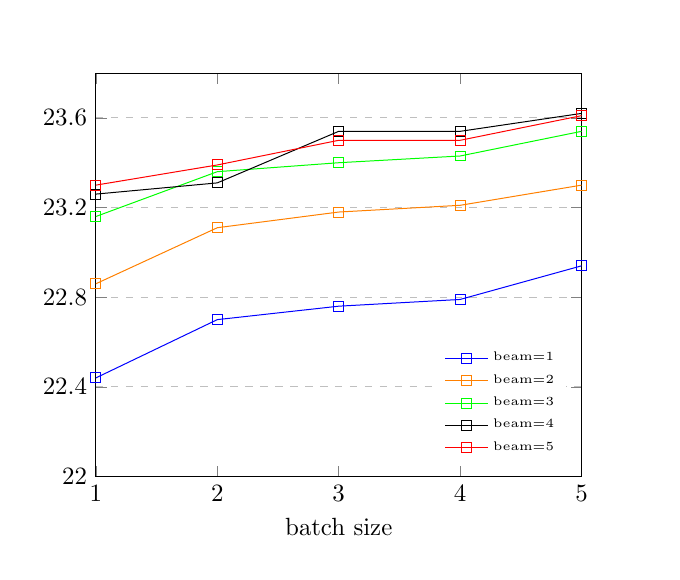
\begin{tikzpicture}
\scalebox{0.9}{
\begin{axis}[
    %title={BLEU},
    xlabel={batch size},
    %ylabel={},
    xmin=1, xmax=5,
    ymin=22, ymax=23.8,
    xtick={1,2,3,4,5},
    ytick={22.0,22.4,22.8,23.2,23.6},
    legend pos=south east,
    %legend style={font=\fontsize{4}{5}\selectfont},
    legend style={font=\tiny, draw=none},
    ymajorgrids=true,
    grid style=dashed,
]
 
\addplot[
    color=blue,
    mark=square,
    ]
    coordinates {
    (1,22.44)	(2,22.7)	(3,22.76)	(4,22.79)	(5,22.94)
    };

\addplot[
    color=orange,
    mark=square,
    ]
    coordinates {
    (1,22.86)	(2,23.11)	(3,23.18)	(4,23.21)	(5,23.3)
    };
    
\addplot[
    color=green,
    mark=square,
    ]
    coordinates {
    (1,23.16)	(2,23.36)	(3,23.4)	(4,23.43)	(5,23.54)
    };

\addplot[
    color=black,
    mark=square,
    ]
    coordinates {
    (1,23.26)	(2,23.31)	(3,23.54)	(4,23.54)	(5,23.62)
    };

\addplot[
    color=red,
    mark=square,
    ]
    coordinates {
    (1,23.3)	(2,23.39)	(3,23.5)	(4,23.5)	(5,23.61)
    };

    \legend{beam=1, beam=2, beam=3, beam=4, beam=5}
 
\end{axis}
}
\end{tikzpicture}
\caption{BLEU evaluations on different beam size and batch size}
\label{fig:beam_batch_bleu}
\end{figure}


At the same time, the decoding cost is increasing when larger beam and batch size are setting (Figure \ref{fig:beam_batch_cpu}).
For beam size 1 (in blue), we process more sentences inside each batch and the CPU cost reduces along the increasing of batch size.
While for the others, larger beam size and larger batch size both cost more computational effort.

As a result, we choose beam 2 and batch 2, balancing the performance and computation cost.

\begin{figure}
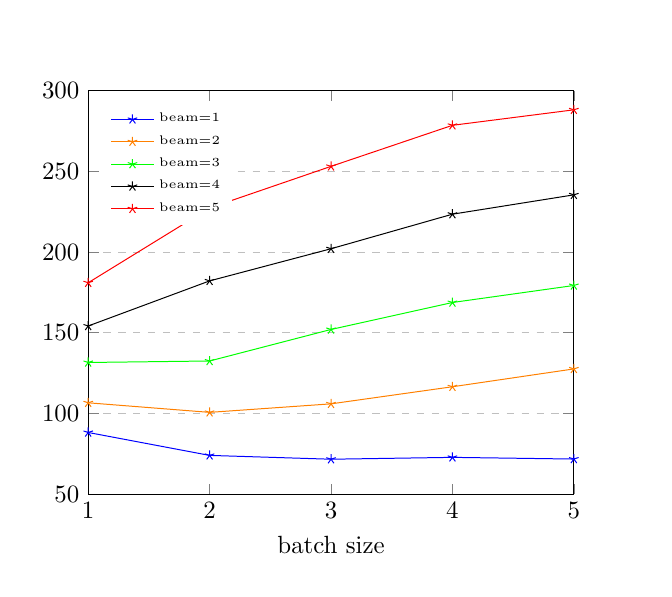
\begin{tikzpicture}
\scalebox{0.9}{
\begin{axis}[
    %title={CPU time},
    xlabel={batch size},
    %ylabel={},
    xmin=1, xmax=5,
    ymin=50, ymax=300,
    xtick={1,2,3,4,5},
    ytick={50,100,150,200,250,300},
    legend pos=north west,
    %legend style={font=\fontsize{4}{5}\selectfont},
    legend style={font=\tiny, draw=none},
    ymajorgrids=true,
    grid style=dashed,
]
 
\addplot[
    color=blue,
    mark=star,
    ]
    coordinates {
    (1,88.2)	(2,74)	(3,71.63)	(4,72.78)	(5,71.74)
    };

\addplot[
    color=orange,
    mark=star,
    ]
    coordinates {
    (1,106.59)	(2,100.66)	(3,105.94)	(4,116.53)	(5,127.58)
    };
    
\addplot[
    color=green,
    mark=star,
    ]
    coordinates {
    (1,131.57)	(2,132.49)	(3,152.02)	(4,168.73)	(5,179.27)
    };

\addplot[
    color=black,
    mark=star,
    ]
    coordinates {
    (1,154.18)	(2,182.12)	(3,202.04)	(4,223.45)	(5,235.43)
    };

\addplot[
    color=red,
    mark=star,
    ]
    coordinates {
    (1,180.97)	(2,227.26)	(3,253.09)	(4,278.52)	(5,288.11)
    };

    \legend{beam=1, beam=2, beam=3, beam=4, beam=5}
 
\end{axis}
}
\end{tikzpicture}
\caption{CPU time (seconds) on different beam size and batch size}
\label{fig:beam_batch_cpu}
\end{figure}


\section{Docker size}
We did not focus on docker image size during the preparation of the submission, and our fastest system docker is 200M for effective 75Mb size for the model and less than 15Mb for additional code and resources. Post-submission, we looked at reducing this 100Mb overhead coming from operating system and found that easy optimizations could be applied - for instance like remove useless dependencies like Python. Without huge effort - we managed to reduced this overhead to 70Mb and it is probably easy to reduce even more.

\section{Further work and Conclusion}

% docker size => -50M
We train through distillation a fat encoder, thin decoder sequence to sequence NMT system for WNMT 2018 running one one single CPU. The models use quantization leading to both a size reduction and a speed gain. Several additional optimizations could have been applied, such as full graph quantization, augmentation of vocabulary size, more improvement on vocabulary mapping...


We need to note that at this level of optimization, especially the use of quantization, makes the speed measurement very dependent on other processes running on the same instance, especially due to the critical importance of the L3/L4-cache shared between the different cores. In particular, we observed that 4 parallel process using fastest model were only reaching a x3 speed boost. To go further on parallel decoding, one would need to implement synchronization points between parallel decoding to avoid waste of memory cache transfer.

%\section*{Acknowledgments}
%
%The acknowledgments should go immediately before the references.  Do not number the acknowledgments section ({\em i.e.}, use \verb|\section*| instead of \verb|\section|). Do not include this section when submitting your paper for review.

% include your own bib file like this:
%\bibliographystyle{acl}
%\bibliography{acl2018}
\bibliography{acl2018}
\bibliographystyle{acl_natbib}

\end{document}

